 \documentclass[12pt]{article}
 \usepackage{cancel}
 \usepackage{multicol}
 \usepackage{amsmath}
 \usepackage{amssymb}
 \usepackage{setspace}
 \usepackage{xcolor}
 \usepackage{graphicx}    % needed for including graphics e.g. EPS, PS
 \usepackage{tikz}
 \usetikzlibrary{patterns,decorations.pathreplacing,shapes,arrows,matrix,positioning}
 \usepackage{3dplot}
 \usepackage[vlined]{algorithm2e}
 \topmargin -2.5cm        % read Lamport p.163
 \oddsidemargin -0.04cm   % read Lamport p.163
 \evensidemargin -0.04cm  % same as oddsidemargin but for left-hand pages
 \textwidth 16.59cm
 \textheight 25.94cm
% \pagestyle{empty}        % Uncomment if don't want page numbers
 \pagenumbering{gobble}
 \parskip 7.2pt           % sets spacing between paragraphs
 %\renewcommand{\baselinestretch}{1.5} 	% Uncomment for 1.5 spacing between lines
 \parindent 0pt		  % sets leading space for paragraphs

% Title
\title{\LARGE\textbf{Chapter 8: Eigenvalues}\normalsize}

% No date in header
\date{}

\newcommand{\inv}[1]{{#1}^{-1}}

\newcommand{\iter}[1]{^{\myp{#1}}}

\newcommand{\lp}{\left(}
\newcommand{\rp}{\right)}
\newcommand{\lb}{\left[}
\newcommand{\rb}{\right]}
\newcommand{\ls}{\left\{}
\newcommand{\rs}{\right\}}
\newcommand{\lbar}{\left|}
\newcommand{\rbar}{\right|}
\newcommand{\ld}{\left.}
\newcommand{\rd}{\right.}

\newcommand{\hs}{\hspace{.75mm}}
\newcommand{\bs}{\hspace{-.75mm}}
\newcommand{\nin}{\noindent}

\newcommand{\fx}{f\bs\left( x \right)}
\newcommand{\gx}{g\bs\left( x \right)}
\newcommand{\qx}{q\bs\left( x \right)}

\newcommand{\nn}{\nonumber}

\newcommand{\vfive}{\vspace{5mm}}
\newcommand{\vthree}{\vspace{3mm}}

\newcommand{\fof}[1]{f\lp #1\rp}
\newcommand{\gof}[1]{g\lp #1\rp}
\newcommand{\qof}[1]{q\lp #1\rp}

\newcommand{\myp}[1]{\left( #1 \right)}
\newcommand{\myb}[1]{\left[ #1 \right]}
\newcommand{\myv}[1]{\left< #1 \right>}
\newcommand{\mys}[1]{\left\{ #1 \right\}}
\newcommand{\myab}[1]{\left| #1 \right|}

\newcommand{\myj}{_j}
\newcommand{\myjp}{_{j+1}}
\newcommand{\myjm}{_{j-1}}

\newcommand{\f}[1]{f\hspace{-1mm}\left( #1 \right)}
\newcommand{\fp}[1]{f'\hspace{-1mm}\left( #1 \right)}
\newcommand{\g}[1]{g\hspace{-1mm}\left( #1 \right)}
\newcommand{\gp}[1]{g'\hspace{-1mm}\left( #1 \right)}
\newcommand{\q}[1]{q\hspace{-1mm}\left( #1 \right)}
\newcommand{\qp}[1]{q'\hspace{-1mm}\left( #1 \right)}
\newcommand{\Px}[1]{P\hspace{-1mm}\left( x_{#1} \right)}
\newcommand{\Qx}[1]{Q\hspace{-1mm}\left( x_{#1} \right)}

\newcommand{\tten}[1]{\times 10^{#1}}

\newcommand{\aij}[1]{a_{#1}}
\newcommand{\bij}[1]{b_{#1}}

\newcommand{\R}[1]{\mathbb{R}^{#1}}
\newcommand{\C}[1]{\mathbb{C}^{#1}}
\newcommand{\F}[1]{\mathbb{F}^{#1}}
\newcommand{\myr}[1]{\textcolor{red}{#1}}

\newcommand{\ith}{i^{\textrm{th}}}
\newcommand{\jth}{j^{\textrm{th}}}
\newcommand{\kth}{k^{\textrm{th}}}

\newcommand{\ben}{\begin{enumerate}}
\newcommand{\een}{\end{enumerate}}

\newcommand{\beq}{\begin{eqnarray}}
\newcommand{\eeq}{\end{eqnarray}}

\tikzset{>=stealth'}

% matrix macro
\newcommand{\mymat}[1]{
\left[
\begin{array}{rrrrrrrrrrrrrrrrrrrrrrrrrrrrrrrrrrrrrrr}
#1
\end{array}
\right]
}


\newcommand{\mydim}[2]{
$#1 \times #2$
}

\newcommand{\myra}{\quad \Rightarrow \quad}

\newcommand{\bS}{\mathbf{S}}
\newcommand{\bw}{\mathbf{w}}
\newcommand{\bx}{\mathbf{x}}
\newcommand{\bX}{\mathbf{X}}
\newcommand{\bd}{\mathbf{d}}
\newcommand{\bdx}{\mathbf{\delta x}}
\newcommand{\bp}{\mathbf{p}}
\newcommand{\bq}{\mathbf{q}}
\newcommand{\bz}{\mathbf{z}}
\newcommand{\bv}{\mathbf{v}}
\newcommand{\bu}{\mathbf{u}}
\newcommand{\by}{\mathbf{y}}
\newcommand{\ba}{\mathbf{a}}
\newcommand{\bb}{\mathbf{b}}
\newcommand{\bc}{\mathbf{c}}
\newcommand{\be}{\mathbf{e}}
\newcommand{\br}{\mathbf{r}}
\newcommand{\bh}{\mathbf{h}}
\newcommand{\bfb}{\mathbf{b}}
\newcommand{\xhat}{\hat{\mathbf{x}}}
\newcommand{\bzero}{\mathbf{0}}

\newcommand{\coker}{\textrm{coker}\hs}
\newcommand{\corange}{\textrm{corng}\hs}
\newcommand{\range}{\textrm{rng}\hs}
\newcommand{\myspan}{\textrm{span}\hs}
\newcommand{\rank}{\textrm{rank}\hs}
\newcommand{\trace}{\textrm{tr}\hs}

\newcommand{\lam}{\lambda}


\tikzstyle{block} = [rectangle, draw, fill=blue!15, text width=6em, text centered, rounded corners, minimum height=4em]
\tikzstyle{line} = [draw, -latex']

\tikzset{main node/.style={circle,fill=blue!20,draw,minimum size=.75cm,inner sep=0pt},
            }

% Actual document starts here
% ======================================================================================
\begin{document}
% \maketitle

% Footer
\let\thefootnote\relax\footnotetext{
\\ Chris Ketelsen
\\ CSCI 2820
\\ Lectures 15 and 16
\\ \today }

% Actual text body starts here
% ======================================================================================

\vspace{-15mm}

% =================================================================================================================
% Lecture 15: Geometry and Intro to Projections
% =================================================================================================================

\nin\Huge{\bf Lecture 15}\normalsize
\vspace{4mm}
\hrule

\vthree

We now take a closer look at the geometry of vectors and it's relationship the fundamental subspaces of a matrix.  The important concepts in his unit include the development of orthogonal bases for the column space of a matrix and their use in data fitting and the very import {\bf least-squares problem}.

\section*{Vector Geometry}

\vthree

\nin The length of a vector can be defined in the usual geometric sense in $\R{2}$ or $\R{3}$.

\begin{center}
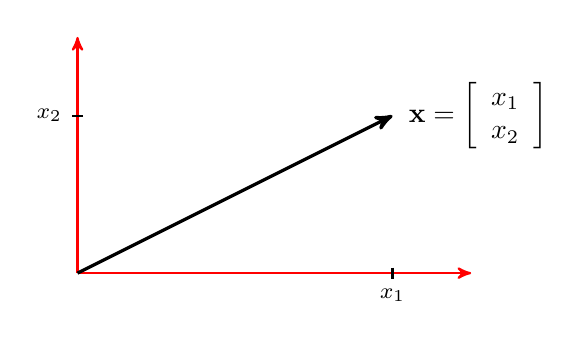
\begin{tikzpicture}[scale=1,
                          axis/.style={thick, red,->},
                          cube/.style={very thick, black},
                          mysolid/.style={very thick, black},
                          mydash/.style={thick, dashed, black},
                         ]


\coordinate (0) at (0,0);

\draw[axis] (0) -- (5,0) node[right]{};
\draw[axis] (0) -- (0,3) node[right]{};

\draw[mysolid, ->] (0,0) -- (4,2) node[right,xshift=2pt]{$\bx = \mymat{x_1 \\ x_2}$};

% \draw[thick] (3.8,1)--(3.8,1.2)--(4,1.2);

\draw[thick] (2pt,2)--(-2pt,2) node[left]{\footnotesize$x_2$\normalsize};
\draw[thick] (4,2pt)--(4,-2pt) node[below]{\footnotesize$x_1$\normalsize};

\end{tikzpicture}
\end{center}

\vthree

\nin From the Pythagorean Theorem we see that the length of the vector $\bx$ is given by $\sqrt{x_1^2 + x_2^2}$.  We denote the length or {\bf norm} of a vector by the following:

\[
\|\bx\| = \sqrt{x_1^2 + x_2^2}
\]

\vthree

\nin The idea of a length of a vector generalizes naturally to vectors in $\R{n}$ despite the fact that we can't picture vectors nor lengths in such high dimensions.  Regardless, we define for $\bx \in \R{n}$:


\[
\|\bx\| = \sqrt{x_1^2 + x_2^2 + \cdots + x_n^2}
\]

\vthree

\nin Notice that the sum of squares inside the square root can also be written as the dot product of $\bx$ with itself.  So we have alternatively

\[
\|\bx\| \hs=\hs \sqrt{x_1^2 + x_2^2 + \cdots + x_n^2} \hs=\hs \sqrt{\bx \cdot \bx} \hs=\hs \sqrt{\bx^T\bx}
\quad \textrm{or} \quad
\|\bx\|^2 = \bx^T\bx
\]

\clearpage

\nin In many applications it's useful to define a vector $\bu$ that points in the same direction as a vector $\bv$ but has length one.   Clearly we can obtain a vector such as this by scaling the vector $\bv$ by the reciprocal of it's length, i.e.

\[
\bu = \frac{\bv}{\|\bv\|}
\]

\nin We call such a vector a {\bf unit vector}.

\vthree

\nin We showed in class previously that two vectors are perpendicular or {\bf orthogonal} if their dot products are zero.  We say $\bu$ and $\bv$ are orthogonal, or $\bu \perp \bv$ if

\[
\bu \cdot \bv = \bu^T \bv = 0
\]

\nin It turns out that the dot product of two vectors can tell us something about their relationship even if they're not orthogonal.  In general the dot product of two vectors is equal to the product of the norms of the vectors and the cosine of the angle between them.
""
\vthree

\nin {\bf Fact}: $\bu \cdot \bw = \|\bu\|\|\bw\| \cos \theta$

\vthree

\nin {\bf Geometric Proof}: Consider vectors $\bv$ and $\bw$ in $\R{2}$ and orient them tail-to-tail along with the difference vector $\bv- \bw$.

\begin{center}
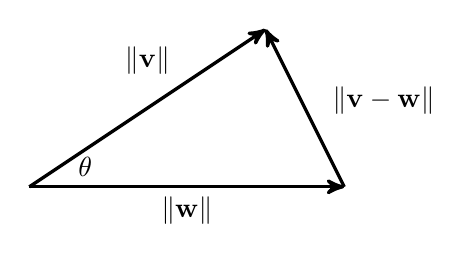
\begin{tikzpicture}[scale=1,
                          axis/.style={thick, red,->},
                          cube/.style={very thick, black},
                          mysolid/.style={very thick, black},
                          mydash/.style={thick, dashed, black},
                         ]


\coordinate (0) at (0,0);

\draw[mysolid, ->] (0,0) -- (3,2);
\draw[mysolid, ->] (0,0) -- (4,0);
\draw[mysolid, ->] (4,0) -- (3,2);
\draw (1.5,1.3) node[above]{$\|\bv\|$};
\draw (2.0,0.0) node[below]{$\|\bw\|$};
\draw (4.5,1.4) node[below]{$\|\bv-\bw\|$};
\draw (0.0,0.0) node[right,xshift=5mm,yshift=2.5mm]{$\theta$};

% \draw[thick] (3.8,1)--(3.8,1.2)--(4,1.2);

% \draw[thick] (2pt,2)--(-2pt,2) node[left]{\footnotesize$x_2$\normalsize};
% \draw[thick] (4,2pt)--(4,-2pt) node[below]{\footnotesize$x_1$\normalsize};

\end{tikzpicture}
\end{center}

\nin Then, from the Law of Cosines we have

\[
\|\bv - \bw\|^2 = \|\bv\|^2 + \|\bw\|^2 - 2\|\bv\|\|\bw\|\cos \theta
\]

\vthree

\nin But from the relationship between the norm and the dot product we have

\beq
\nn \|\bv - \bw\|^2 &=& \myp{\bv-\bw}^T\myp{\bv-\bw} \\
\nn                 &=& \bv^T\bv - 2\bv^T\bw + \bw^T\bw \\
\nn                 &=& \|\bv\|^2 - 2\bv^T\bw + \|\bw\|^2
\eeq

\clearpage

\nin Setting the right-hand side of these two identities equal to each other we have

\[
\|\bv\|^2 + \|\bw\|^2 - 2\|\bv\|\|\bw\|\cos \theta =  \|\bv\|^2 - 2\bv^T\bw + \|\bw\|^2
\]

\nin and canceling like terms on either side gives

\[
\|\bv\|\|\bw\|\cos \theta =  \bv^T\bw.
\]

\hfill $\square$

\clearpage

The cosine formula tells us several things about how the dot product of two vectors relates to their orientation to one another.

\vthree

\nin First, if we fix the lengths of $\bv$ and $\bw$ and consider how the dot product changes as the angle between them changes, we see that the dot product takes on it's maximum positive value when the vectors are parallel and point in the same direction.  In this case we have $\theta = 0$ and

\[
\bv^T\bw = \|\bv\|\|\bw\|\cos\myp{0} = \|\bv\|\|\bw\|
\]

\vthree

\nin Second, the dot product of vectors $\bv$ and $\bw$ takes on it largest negative value when the vectors are parallel but pointed in opposite directions.  In this case we have $\theta = \pi$ and

\[
\bv^T\bw = \|\bv\|\|\bw\|\cos\myp{\pi} = -\|\bv\|\|\bw\|
\]

\vthree

\nin Finally, we see that if the angle takes on any other value in between the dot product will be of smaller magnitude.  In general the dot product will be positive if the vectors point in generally the same direction (the angle less than perpendicular) and will be negative if the vectors point in generally differing directions (the angle is passed perpendicular).

\vthree

\begin{minipage}{.33\textwidth}
\begin{center}
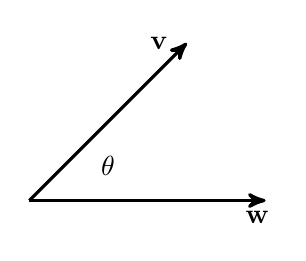
\begin{tikzpicture}[scale=1,
              axis/.style={thick, red,->},
              cube/.style={very thick, black},
              mydash/.style={thick, dashed, black},
             ]
\coordinate (center) at (0,0);
\draw[very thick, ->] (0,0) -- (2,2) node[left,xshift=-3pt]{$\bv$};
\draw[very thick, ->] (0,0) -- (3,0) node[below,xshift=-3pt]{$\bw$};
\draw (1,.2) node[above]{$\theta$};
\end{tikzpicture}

\normalsize$\theta$ acute $\Rightarrow$ $\bv\cdot\bw > 0$ \normalsize

\end{center}
\end{minipage}
\begin{minipage}{.33\textwidth}
\begin{center}
\begin{tikzpicture}[scale=1,
              axis/.style={thick, red,->},
              cube/.style={very thick, black},
              mydash/.style={thick, dashed, black},
             ]
\coordinate (center) at (0,0);
\draw[very thick, ->] (0,0) -- (-1,2) node[left,xshift=-3pt]{$\bv$};
\draw[very thick, ->] (0,0) -- (3,0) node[below,xshift=-3pt]{$\bw$};
\draw (.4,.2) node[above]{$\theta$};
\end{tikzpicture}

$\theta$ obtuse $\Rightarrow$ $\bv\cdot\bw < 0$

\end{center}
\end{minipage}
\begin{minipage}{.33\textwidth}
\begin{center}
\begin{tikzpicture}[scale=1,
              axis/.style={thick, red,->},
              cube/.style={very thick, black},
              mydash/.style={thick, dashed, black},
             ]
\coordinate (center) at (0,0);
\draw[very thick, ->] (0,0) -- (0,2) node[left,xshift=-3pt]{$\bv$};
\draw[very thick, ->] (0,0) -- (3,0) node[below,xshift=-3pt]{$\bw$};
\draw (.4,.2) node[above]{$\theta$};
\end{tikzpicture}

$\theta=90^\circ$ $\Rightarrow$ $\bv\cdot\bw = 0$

\end{center}
\end{minipage}


\vthree

\nin {\bf Rule of Thumb}: The dot product of two vectors tell us generally how much two vectors align with one another.

\vthree

\nin From this definition of the dot product we have two very import inequalities:

\vthree

\nin {\bf Schwarz's Inequality}: $\myab{\bv \cdot \bw} \leq \|\bv\|\|\bw\|$

\vthree

\nin {\bf Proof}:  The proof follows immediately from the cosine formula for dot products and the fact that the cosine function is always between minus one and one.  Taking the absolute value of the dot product gives

\[
\myab{\bv \cdot \bw} = \|\bv\|\|\bw\|\myab{\cos \theta} \leq \|\bv\|\|\bw\|
\]

\hfill $\square$

\clearpage

\nin {\bf The Triangle Inequality}: $\|\bv + \bw\| \leq \|\bv\| + \|\bw\|$

\vthree

\nin In class we did a handwavy geometric proof of the Triangle Inequality.  Here we give an algebraic proof that relies on Schwarz's Inequality.

\vthree

\nin {\bf Proof}:  Note that since all of the terms in the inequality are positive it is still true if we square both sides.  So instead we'll prove the equivalent statement

\[
\|\bv + \bw\|^2 \leq \myp{\|\bv\| + \|\bw\|}^2
\]

\nin Starting with the left-hand side, we have

\beq
\nn \|\bv + \bw\|^2 &=& \myp{\bv + \bw}^T\myp{\bv + \bw} \\
\nn &=& \|\bv\|^2 + 2\bv^T\bw + \|\bw\|^2
\eeq

\vthree

\nin Now note that it's possible the dot product of $\bv$ and $\bw$ is negative.  So if we throw absolute values around it it can only make the expression on the right-hand side of the equation larger.  Thus we have

\beq
\nn \|\bv + \bw\|^2 &=& \myp{\bv + \bw}^T\myp{\bv + \bw} \\
\nn &=& \|\bv\|^2 + 2\bv^T\bw + \|\bw\|^2 \\
\nn &\leq& \|\bv\|^2 + 2\myab{\bv^T\bw} + \|\bw\|^2 \\
\nn &\leq& \|\bv\|^2 + 2\|\bv\|\|\bw\| + \|\bw\|^2 \\
\nn &=& \myp{\|\bv\| + \|\bw\|}^2
\eeq

\vthree

\nin where the second-to-last line follows from Schwartz's Inequality and the last line comes from factoring.

\hfill $\square$

\clearpage

\section*{Projections}

\vthree

\nin As we start to talk about the least-squares problem, the notion of the {\it closest vector to a subspace} will become immensely important.  Suppose that we have a vector $\bfb$ and a one-dimensional subspace of $\R{3}$ (a.k.a. a line) spanned by a single vector $\ba$.  If the vector $\bfb$ does not lie along the line then we might ask What is the vector that lies on the line that is in some sense {\it closest} to the vector $\bfb$?

\nin This closest vector is called the projection of $\bfb$ onto the subspace representing the line and is denoted as the vector $\bp$.  You can think of the projection vector $\bp$ as the shadow that the vector $\bfb$ would make on the line if you shined a flashlight on the vector $\bfb$ and perpendicular to the line.

\begin{center}
\begin{tikzpicture}[scale=1,rotate=-15,
              axis/.style={thick, red,->},
              cube/.style={very thick, black},
              mydash/.style={thick, dashed, black},
             ]

\coordinate (center) at (0,0);

\draw[very thick, ->] (0,0) -- (2,2) node[above,xshift=-5pt,yshift=1pt]{\footnotesize$\bfb$\normalsize};
\draw[very thick] (-3,0) -- (5,0) node[right,xshift=-3pt,yshift=-2pt,rotate=-15]{$L = \textrm{span}\mys{\ba}$};
\draw[cyan, very thick, ->] (0,0) -- (2,0);
\draw (2,0) node[below,xshift=-25pt,yshift=2mm,rotate=-15]{$\bp$};
\draw[thick, dashed]  (2,2) -- (2,0);
\draw[very thick]  (1.7,0) -- (1.7,0.3) -- (2,0.3);
\draw[very thick] (1.8,4.0) -- (2.2,4.0) -- (2.2,3.2) -- (2.35,3.0) -- (1.65,3.0) -- (1.8,3.2) -- (1.8,4);
\draw[very thick] (2,3.0) -- (2,2.7);
\draw[very thick] (1.8,3.0) -- (1.8,2.8);
\draw[very thick] (2.2,3.0) -- (2.2,2.6);
\end{tikzpicture}
\end{center}

\vthree

\nin Note that the projection vector $\bp$ lies {\bf in} the subspace of the line and points in the same general direction as $\bfb$.

\vthree

\nin We can also talk about projecting vectors into higher dimensional subspaces as well, such as planes.  Consider the following example.


\clearpage

\nin {\bf Example 1}:  Find the projection of the vector $\bfb = \myb{\hs 1, \hs 4, \hs 2\hs}^T$ onto (1) the $z-$axis and (2) the $xy$-plane.

\vthree

\nin Using the flashlight and shadow analogy it's easy to see that the projection of $\bfb$ onto the $z$-axis is the vector $\bp_1 = \myb{\hs 0 ,\hs 0 ,\hs 2 \hs}^T$ and the projection of $\bfb$ onto the $xy$-plane is the vector $\bp_2 = \myb{\hs 1 ,\hs 4 ,\hs 0 \hs}^T$.

\tdplotsetmaincoords{60}{120}

\begin{center}
\begin{tikzpicture}[scale=2,
              tdplot_main_coords,
              axis/.style={thick, red,->},
              cube/.style={very thick, black},
              mydash/.style={very thin, dashed, black},
             ]

\coordinate (0) at (0,0,0);

\draw[axis] (0) -- (3,0,0) node[anchor=north east]{$x$};
\draw[axis] (0,0,0) -- (0,5,0) node[anchor=north west]{$y$};
\draw[axis] (0,0,0) -- (0,0,3) node[anchor=south]{$z$};

\draw[very thick, ->] (0,0,0) -- (1,4,2) node[right]{$\bfb$};
\draw[very thick, cyan, ->] (0,0,0) -- (0,0,2) node[right,yshift=2mm,black]{$\bp_1$};
\draw[very thick, cyan, ->] (0,0,0) -- (1,4,0) node[right,xshift=2mm,black]{$\bp_2$};

\draw[mydash] (1,0,0) -- (1,4,0) -- (0,4,0);
\draw[mydash] (1,0,2) -- (1,4,2) -- (0,4,2) -- (0,0,2) -- cycle;
\draw[mydash] (0,4,0) -- (0,4,2);
\draw[mydash] (1,4,0) -- (1,4,2);
\draw[mydash] (1,0,0) -- (1,0,2);

\draw[very thick, red] (-.075,1,0) -- (.075,1,0);
\draw[very thick, red] (-.075,2,0) -- (.075,2,0);
\draw[very thick, red] (-.075,3,0) -- (.075,3,0);
\draw[very thick, red] (-.075,4,0) -- (.075,4,0);

\draw[very thick, red] (1,-.075,0) -- (1,.075,0);

\draw[very thick, red] (0,-.075,1) -- (0,.075,1);
\draw[very thick, red] (0,-.075,2) -- (0,.075,2);

% \draw (2,0,0) node[xshift=-5pt,yshift=5pt]{\footnotesize$a$\normalsize};
% \draw (0,2,0) node[xshift=5pt,yshift=5pt]{\footnotesize$b$\normalsize};
% \draw (0,0,2) node[xshift=-5pt,yshift=1pt]{\footnotesize$c$\normalsize};

\end{tikzpicture}
\end{center}

\vthree

\nin Note that in each case the projection vector $\bp$ lies {\bf in} the subspace that $\bfb$ was projected onto.

\vthree

\nin It is often useful to think of the projection operation as the operation of a matrix on the vector $\bfb$.  In general, we want to write

\[
\bp = P \bfb
\]

\vthree

\nin where $P$ is the so-called {\bf projection matrix}.  For this example, we'd like to find matrices $P_1$ and $P_2$ such that

\[
P_1 \mymat{1 \\ 4 \\ 2} = \mymat{0 \\ 0 \\ 2} \quad \textrm{and} \quad
P_2 \mymat{1 \\ 4 \\ 2} = \mymat{1 \\ 4 \\ 0}
\]

\vthree

\nin For this simple example it's very easy to see that the projection matrices that project onto the $z$-axis and $xy$-plane, respectively, are

\[
P_1 =
\mymat{
0 & 0 & 0 \\
0 & 0 & 0 \\
0 & 0 & 1 \\
}
\quad \textrm{and} \quad
P_2 =
\mymat{
1 & 0 & 0 \\
0 & 1 & 0 \\
0 & 0 & 0 \\
}
\]

\vthree

\nin Note that because the two subspaces we've projected onto are orthogonal subspaces, we have the nice result that

\[
\bp_1 + \bp_2 = \mymat{0 \\ 0 \\ 2} + \mymat{1 \\ 4 \\ 0} = \mymat{1 \\ 4 \\ 2} = \bfb
\quad \textrm{and} \quad
P_1 + P_2 = I
\]

\hfill $\square$

\vthree

\nin Referring to the subspaces projected onto as axes and coordinate planes is pretty easy in three dimensions, but with more complicated and higher dimensional subspaces we need a more systematic method to describe the space.  Notice that in both of the cases in the previous example, instead of talking about projecting onto a geometric space, we can talk about projecting onto the column space of a matrix.  For example, projecting onto the $z$-axis is equivalent to projecting onto the column space of

\[
A_1 = \mymat{0 \\ 0 \\ 1} \quad \textrm{or} \quad A_1 = \mymat{0 \\ 0 \\ 2}.
\]

\vthree

\nin Similarly projecting onto the $xy$-plane is equivalent to projecting onto the column space of

\[
A_2 = \mymat{1 & 0 \\ 0 & 1 \\ 0 & 0 } \quad \textrm{or} \quad A_2 = \mymat{1 & 1 \\ 1 & -1 \\ 0 & 0}.
\]

\vthree

\section*{Projection onto a Line}

\vthree

\nin Now we'll look at the process of projecting onto a line (a one-dimensional subspace) in greater detail.  Suppose we want to find the projection $\bp$ of the vector $\bp$ onto the subspace spanned by the vector $\ba$.  The general picture looks as follows

\tdplotsetmaincoords{75}{120}

\begin{center}
\begin{tikzpicture}[scale=2,
              tdplot_main_coords,
              axis/.style={thick, red,->},
              cube/.style={very thick, black},
              mydash/.style={very thin, dashed, black},
             ]

\coordinate (0) at (0,0,0);

\draw[axis] (0) -- (3,0,0) node[anchor=north east]{$x$};
\draw[axis] (0,0,0) -- (0,4,0) node[anchor=north west]{$y$};
\draw[axis] (0,0,0) -- (0,0,3) node[anchor=south]{$z$};

\draw[thick, dashed] (0,0,0) -- (5,5,5) node[right]{$\textrm{span}\mys{\ba}$};
\draw[very thick, cyan, ->] (0,0,0) -- (2.33,2.33,2.33) node[left]{$\bp$};
\draw[very thick, red, ->] (2.33,2.33,2.33) -- (1,4,2) node[right]{};
\draw[very thick, ->] (0,0,0) -- (1,4,2) node[right]{$\bfb$};
\draw[very thick, ->] (0,0,0) -- (1,1,1) node[right]{$\ba$};
\draw (1.75, 3.5, 2.2) node[above]{${\textcolor{red}\be} = \bfb - {\textcolor{cyan}\bp}$};
% \draw[very thick, cyan, ->] (0,0,0) -- (0,0,2) node[right,yshift=2mm,black]{$\bp_1$};
% \draw[very thick, cyan, ->] (0,0,0) -- (1,4,0) node[right,xshift=2mm,black]{$\bp_2$};

% \draw[mydash] (1,0,0) -- (1,4,0) -- (0,4,0);
% \draw[mydash] (1,0,2) -- (1,4,2) -- (0,4,2) -- (0,0,2) -- cycle;
% \draw[mydash] (0,4,0) -- (0,4,2);
% \draw[mydash] (1,4,0) -- (1,4,2);
% \draw[mydash] (1,0,0) -- (1,0,2);

% \draw[very thick, red] (-.075,1,0) -- (.075,1,0);
% \draw[very thick, red] (-.075,2,0) -- (.075,2,0);
% \draw[very thick, red] (-.075,3,0) -- (.075,3,0);
% \draw[very thick, red] (-.075,4,0) -- (.075,4,0);

% \draw[very thick, red] (1,-.075,0) -- (1,.075,0);

% \draw[very thick, red] (0,-.075,1) -- (0,.075,1);
% \draw[very thick, red] (0,-.075,2) -- (0,.075,2);

% \draw (2,0,0) node[xshift=-5pt,yshift=5pt]{\footnotesize$a$\normalsize};
% \draw (0,2,0) node[xshift=5pt,yshift=5pt]{\footnotesize$b$\normalsize};
% \draw (0,0,2) node[xshift=-5pt,yshift=1pt]{\footnotesize$c$\normalsize};

\end{tikzpicture}
\end{center}

\vthree

\nin Notice that the vector $\be = \bfb - \bp$ is the difference between the original vector $\bfb$ and the projection vector $\bp$.  Notice also that if the projection vector $\bp$ is really the vector on the line that is closest to $\bfb$ then the difference vector $\be$ will be orthogonal to $\bp$.  We label the difference vector $\be$ because it can be thought of as the {\bf error} made if we approximate the vector $\bfb$ by its projection $\bp$.

\vthree

\nin OK, so how do we compute the projection vector $\bp$ given the original vector $\bfb$ and the vector $\ba$ that describes the line?

\vthree

\nin Note that the projection $\bp$ is in the subspace $\textrm{span}\mys{\ba}$ which means it can be written as a scalar multiple of $\ba$.  Let the (as yet unknown) multiplier by $\hat{x}$, then we have

\[
\bp = \hat{x}\ba
\]

\nin Remember that we said that $\bp$ is the vector in $\textrm{span}\mys{\ba}$ that makes the error vector $\be = \bfb - \bp$ orthogonal to $\ba$.  We can enforce this condition by dotting $\be$ by $\ba$ and setting it to zero.  We then find the correct multiplier $\hat{x}$ that makes the equation true.

\beq
\nn 0 &=& \ba^T\myp{\bfb - \hat{x}\ba} \\
\nn 0 &=& \ba^T\bfb - \hat{x}\ba^T\ba \\
\nn \hat{x}\ba^T\ba &=& \ba^T\bfb \\
\nn \hat{x} &=& \frac{\ba^T\bfb}{\ba^T\ba}
\eeq

\vthree

\nin So we have

\[
\hat{x} = \frac{\ba^T\bfb}{\ba^T\ba} \quad \textrm{and so} \quad \bp = \frac{\ba^T\bfb}{\ba^T\ba} \ba
\]

\vthree

\nin {\bf Example 2}: Compute the projection of $\bfb = \mymat{1 \\ 4 \\ 2}$ onto the subspace spanned by $\ba = \mymat{0 \\ 0 \\ 1}$

\vthree

\nin We have $\ba^T\bb = 2$ and $\ba^T\ba = 1$ which gives $\bp = \dfrac{2}{1}\ba = \mymat{0 \\ 0 \\ 2}$

\vthree

\nin What if we had chosen another basis vector for the subspace, for instance $\ba = \mymat{0 \\ 0 \\ 3}$?

\vthree

\nin Then $\ba^T\bb = 6$ and $\ba^T\ba = 9$ which gives $\bp = \dfrac{6}{9}\ba = \mymat{0 \\ 0 \\ 2}$

\clearpage

\nin Hopefully this isn't surprising.  We made the entries of $\ba$ larger, which in turn made $\ba^T\bb$ larger in the numerator, but also made $\ba^T\ba$ comparatively larger in the denominator to compensate.  In general you can use any nonzero basis vector in the subspace for the line and the formula will work.

\hfill $\square$

\vthree

\nin {\bf Example 3}: Compute the projection of $\bfb = \mymat{1 \\ 4 \\ 2}$ onto the subspace spanned by $\ba = \mymat{1 \\ 1 \\ 1}$

\vthree

\nin We have $\ba^T\bb = 7$ and $\ba^T\ba = 3$ which gives $\bp = \dfrac{7}{3}\ba = \mymat{7/3 \\ 7/3 \\ 7/3}$

\vthree

\nin Let's look at some special cases and check the formula as well as our intuition.

\vthree

\nin {\bf $\bb$ already in subspace}: Suppose that $\bb$ is already in $\textrm{span}\mys{\ba}$.  Then clearly the closest vector to $\bb$ in the subspace is $\bb$ itself, so the projection shouldn't change anything.  If $\bb$ is in the subspace we have $\bb = \alpha \ba$ for some scalar $\alpha$.  Then

\[
\ba^T\bb = \ba^T \myp{\alpha \ba} = \alpha \hs \ba^T\ba \quad \textrm{then} \quad \bp = \frac{\alpha \ba^T\ba}{\ba^T\ba}\ba = \alpha\ba = \bb \quad \checkmark
\]

\vthree

\nin {\bf $\bb$ orthogonal to subspace}:  Suppose that $\bb$ is orthogonal to $\textrm{span}\mys{\ba}$.  Then $\bb$ is orthogonal to any vector in $\textrm{span}\mys{\ba}$ and in particular $\bb$ is orthogonal to $\ba$.  Then

\[
\bp = \frac{\ba^T\bb}{\ba^T\ba}\ba = \frac{0}{\ba^T\ba}\ba = {\bf 0}
\]

\nin This should make intuitive sense.  Suppose you projected a vector $\bb$ that lies in the $xy$-plane onto the $z$-axis.  Since the vector $\bb$ does not have any height off the plane, its shadow on the $z$-axis would be nonexistant.

\vthree

\nin OK, so how do we come up with the projection matrix $P$ such that $\bp = P\bb$?

\vthree

\nin Well, we've already done most of the work.  Finding the $P$ matrix just takes some creative rearranging of our formula.  Switching the order of the multiplication in the formula (which is fine, because $\hat{x}$ is just a scalar) gives

\[
\bp = \ba\frac{\ba^T\bb}{\ba^T\ba} = \frac{\ba\ba^T}{\ba^T\ba}\bb = \myp{\frac{\ba\ba^T}{\ba^T\ba}}\bb = P\bb \quad \textrm{so} \quad P = \frac{\ba\ba^T}{\ba^T\ba}
\]

\vthree

\nin Note that the numerator in the expression for $P$ is the {\bf outer-product} of $\ba$ with itself, which is a matrix.

\clearpage

\nin {\bf Example 4}: Compute the projection matrix $P$ for the space $\textrm{span}\mys{\ba}$ with $\ba = \mymat{ 0 \\ 0 \\ 1}$.

\vthree

\nin We have $\ba^T\ba = 1$ and

\[
\ba\ba^T =
\mymat{
0 \\ 0 \\ 1
}
\mymat{0 & 0 & 1}
=
\mymat{
0 & 0 & 0 \\
0 & 0 & 0 \\
0 & 0 & 1 \\
}
\quad \Rightarrow \quad
P =
\mymat{
0 & 0 & 0 \\
0 & 0 & 0 \\
0 & 0 & 1 \\
}
\quad \checkmark
\]

\nin {\bf Example 5}: Compute the projection matrix $P$ for the space $\textrm{span}\mys{\ba}$ with $\ba = \mymat{ 1 \\ 1 \\ 1}$.

\vthree

\nin We have $\ba^T\ba = 3$ and

\[
\ba\ba^T =
\mymat{
1 \\ 1 \\ 1
}
\mymat{1 & 1 & 1}
=
\mymat{
1 & 1 & 1 \\
1 & 1 & 1 \\
1 & 1 & 1 \\
}
\quad \Rightarrow \quad
P =
\frac{1}{3}
\mymat{
1 & 1 & 1 \\
1 & 1 & 1 \\
1 & 1 & 1 \\
}
\]

\nin We can check that multiplication by this $P$ gives us the same projection vector we found in Example 3:

\[
P\bb =
\frac{1}{3}
\mymat{
1 & 1 & 1 \\
1 & 1 & 1 \\
1 & 1 & 1 \\
}
\mymat{1 \\ 4 \\ 2}
= \frac{1}{3}
\mymat{
7 \\ 7 \\ 7
}
= \mymat{7/3 \\ 7/3 \\ 7/3}
\]

\clearpage

% =================================================================================================================
% Lecture 16: Projections in higher dimensional subspaces
% =================================================================================================================

\nin\Huge{\bf Lecture 16}\normalsize
\vspace{4mm}
\hrule

\vthree

\nin Last time we developed a general formula for projecting a vector onto a one-dimensional subspace (i.e. a line).  Now we'll look at the general procedure for projecting a vector into higher dimensional subspaces.  The projection into the $xy$-plane that we looked at in the previous lecture is an example of projecting a vector in $\R{3}$ into a two-dimensional subspace.  We'll consider general $n$-dimensional subspaces here, but keep the plane example in the back of your mind.

\vthree

\nin Suppose we have a basis for an $n$-dimensional subspace of $\R{m}$ and a vector $\bb \in \R{m}$ that we'd like to project.  The projection will have potential contributions from each of the basis vectors, which we'll denote $\ba_1, \ba_2, \ldots, \ba_n \in \R{m}$.

\vthree

\nin Since we know the projection vector $\bp$ must lie in the subspace, it must be possible to write it as a linear combination of the basis vectors, i.e.

\[
\bp = \hat{x}_1 \ba_1 + \hat{x}_2 \ba_2 + \cdots + \hat{x}_n \ba_n
\]

\vthree

\nin Notice that this linear combination of basis vectors kinda looks like the column-view of a matrix vector product.  In fact, the whole process becomes much simpler if we organize the basis vectors into a matrix, $A = \myb{\hs \ba_1 \hs \ba_2 \hs \cdots \hs \ba_n \hs}$, and the unknown $\hat{x}$'s into a vector $\hat{\bx} = \myb{\hs\hat{x}_1, \hs\hat{x}_2, \ldots, \hs\hat{x}_n\hs}^T$.  We then can write the projection vector as

\[
\bp = A\hat{\bx}
\]

\vthree

\nin Note that not much as changed from the one-dimensional case.  We still want to

\ben
\item Find the unknown vector of coefficients $\hat{\bx}$
\item Compute the projection vector $\bp = A\hat{\bx}$
\item Find a projection matrix $P$ such that $\bp = P\bb$
\een

\clearpage

\nin Let's go back to the $xy$-plane projection case to get a better picture of what's going on

\tdplotsetmaincoords{70}{120}

\begin{center}
\begin{tikzpicture}[scale=2,
              tdplot_main_coords,
              axis/.style={thick, red,->},
              cube/.style={very thick, black},
              mydash/.style={very thin, dashed, black},
             ]

\coordinate (0) at (0,0,0);

\draw[axis] (0) -- (3,0,0) node[anchor=north east]{$x$};
\draw[axis] (0,0,0) -- (0,4,0) node[anchor=north west]{$y$};
\draw[axis] (0,0,0) -- (0,0,2) node[anchor=south]{$z$};

\draw[very thick, ->] (0,0,0) -- (2,3,2) node[right]{$\bfb$};
\draw[very thick, ->] (0,0,0) -- (1,0,0) node[above, yshift=1mm]{$\ba_1$};
\draw[very thick, ->] (0,0,0) -- (0,1,0) node[above]{$\ba_2$};
\draw[very thick, cyan, ->] (0,0,0) -- (2,3,0) node[right,xshift=2mm,black]{$\bp$};

\draw[very thick, red, ->] (2,3,0) -- (2,3,2) node[right]{};
\draw (2, 3, 1) node[right]{${\textcolor{red}\be} = \bfb - {\textcolor{cyan}\bp}$};

\draw[mydash] (2,0,0) -- (2,3,0) -- (0,3,0);

\draw[thick, black] (2,3,0.2) -- (1.8,3,0.2) -- (1.8,3,0);

\end{tikzpicture}
\end{center}

\vthree

\nin The picture is very similar as before.  We see that the projection vector $\bp$ is closest to $\bb$ exactly when the error vector $\be = \bb - \bp = \bb - A\hat{\bx}$ is orthogonal to the $xy$-plane.  Our strategy will be to enforce the condition that $\be$ is orthogonal to the subspace and then use the resulting equations to solve for the unknown $\hat{x}$'s.

\vthree

\nin Recall that to enforce that a vector is orthogonal to a subspace it is sufficient to enforce that the vector is orthogonal to each of the basis vectors for the subspace.  In the general $n$-dimensional case we have the basis $\ba_1, \ba_2, \ldots, \ba_n$.  Enforcing that $\be = \bb - A\hat{\bx}$ is orthogonal to each of these gives the following equation

\beq
\nn \ba_1^T\myp{\bb - A\hat{\bx}} &=& 0 \\
\nn \ba_2^T\myp{\bb - A\hat{\bx}} &=& 0 \\
\nn &\vdots& \\
\nn \ba_n^T\myp{\bb - A\hat{\bx}} &=& 0
\eeq

\vthree

\nin Now notice that each of the expressions is a dot product of a column of $A$ with the error vector $\myp{\bb - A\hat{\bx}}$.  Since the columns of $A$ are the rows of $A^T$ we can also say that each expression is the dot dot product of a row of $A^T$ with the the error vector $\myp{\bb - A\hat{\bx}}$.  This is exactly the matrix-vector product of $A^T$ with $\hat{\bx}$.  So an equivalent set of equations is

\[
A^T\myp{\bb - A\hat{\bx}} = {\bf 0}
\]

\vthree

\nin So the vector of coefficients $\hat{\bx}$ that give us the projection vector is the vector $\hat{\bx}$ that solves this system of equations.  Rearranging the system we have


\[
A^T\myp{\bb - A\hat{\bx}} = {\bf 0}
\quad \Rightarrow \quad
A^T\bb - A^TA\hat{\bx} = {\bf 0}
\quad \Rightarrow \quad
A^TA\hat{\bx} = A^T\bb
\]

\clearpage

\nin{\bf Take-Away}: To find the vector of unknown coefficients that give the projection vector we can solve the system of equations $A^TA\hat{\bx} = A^T\bb$ for $\hat{\bx}$.  Then to find the projection vector we form $\bp = A\hat{\bx}$.

\vthree

\nin The system of equations $A^TA\hat{\bx} = A^T\bb$ are called the {\bf normal equations} because they arise from enforcing the conditions that the error vector is orthogonal to the column space of $A$ and another word for orthogonal is {\bf normal}.  Note that if $A$ is an $m \times n$ matrix then the matrix $A^TA$ that must be solved when solving the normal equations is $n \times n$.  It turns out that because the columns of $A$ are a basis for the subspace (and hence linearly independent) that the matrix $A^TA$ is always nonsingular, and thus the normal equations always have a unique solution $\hat{\bx}$ (see a proof of this at the end of this lecture).

\vthree

\nin OK, since $A^TA$ is nonsingular, its inverse $\myp{A^TA}^{-1}$ exists, and we can write the projection vector $\bp$ as

\[
\hat{\bx} = \myp{A^TA}^{-1}A^T\bb
\quad \Rightarrow \quad
\bp = A\hat{\bx}
\quad \Rightarrow \quad
\bp = A\myp{A^TA}^{-1}\bs\bs A^T\bb
\]

\vthree

\nin From this expression it's easy to see that the form of the projection matrix is


\[
P = A\myp{A^TA}^{-1}\bs\bs A^T
\]

\vthree

\nin It's instructive to check that the formula for the harder $n$-dimensional case reduces to the formula we worked out for projecting a vector onto a one-dimensional subspace.  In that case we have just $A = \ba$, and the formula gives

\[
P = \ba\myp{\ba^T\ba}^{-1}\bs\bs\ba^T = \frac{\ba\ba^T}{\ba^T\ba} \quad \checkmark
\]

\vthree

\nin {\bf Example 1}: Find the projection matrix $P$ that projects a vector in $\R{3}$ into the $xy$-plane.

\vthree

\nin We need a matrix $A$ whose columns form a basis for the $xy$-plane.  We'll start with with the most obvious choice:

\[
A = \mymat{
1 & 0 \\
0 & 1 \\
0 & 0 \\
}
\quad \Rightarrow \quad
A^TA = \mymat{
1 & 0 & 0  \\
0 & 1 & 0 \\
}
\mymat{
1 & 0 \\
0 & 1 \\
0 & 0 \\
}
=
\mymat{
1 & 0   \\
0 & 1   \\
}
= I
\]

\vthree

\nin Plugging into the formula we have

\[
P = A\myp{A^TA}^{-1}\bs\bs A^T = AI^{-1}\bs A^T = AA^T =
\mymat{
1 & 0 & 0  \\
0 & 1 & 0 \\
0 & 0 & 0 \\
}
\quad \checkmark
\]

\clearpage

\nin Alternatively we could use a more interesting basis for the $xy$-plane with $A = \mymat{1 & 1 \\ 1 & 2 \\ 0 & 0}$.

\[
A^TA = \mymat{
1 & 1 & 0  \\
1 & 2 & 0 \\
}
\mymat{
1 & 1 \\
1 & 2 \\
0 & 0 \\
}
=
\mymat{
2 & 3   \\
3 & 5   \\
}
\quad \Rightarrow \quad
\myp{A^TA}^{-1} =
\mymat{
5 & -3 \\
-3 & 2
}
\]

\vthree

\[
P = A\myp{A^TA}^{-1}\bs\bs A^T =
\mymat{
1 & 1 \\
1 & 2 \\
0 & 0 \\
}
\mymat{
5 & -3 \\
-3 & 2
}
\mymat{
1 & 1 & 0  \\
1 & 2 & 0 \\
}
=
\mymat{
1 & 1 \\
1 & 2 \\
0 & 0 \\
}
\mymat{
2 &-1 & 0  \\
-1 & 1 & 0 \\
}
=
\mymat{
1 & 0 & 0  \\
0 & 1 & 0 \\
0 & 0 & 0 \\
}
\]

\vthree

\nin {\bf Example 2}: Find the projection of $\bb = \mymat{6 \\ 0 \\ 0}$ onto the column space of $A = \mymat{1 & 0 \\ 1 & 1 \\ 1 & 2}$.

\vthree

\nin Let's do this one is two ways.  First we'll solve the normal equations for $\hat{\bx}$ and for $\bp = A\hat{\bx}$.  Then we'll build the projection matrix $P$ and use it to compute the projection.  We have

\[
A^TA =
\mymat{
1 & 1 & 1 \\
0 & 1 & 2
}
\mymat{
1 & 0 \\
1 & 1 \\
1 & 2
} =
\mymat{
3 & 3 \\
3 & 5
}
\quad \quad
A^T\bb =
\mymat{
1 & 1 & 1 \\
0 & 1 & 2
}
\mymat{6 \\ 0 \\ 0}
= \mymat{6 \\ 0}
\]

\vthree

\nin Solving the augmented system for $\hat{\bx}$ gives

\[
\left[
\begin{array}{rr|r}
3 & 3 & 6 \\
3 & 5 & 0
\end{array}
\right]
\hs\hs \sim \hs\hs
\left[
\begin{array}{rr|r}
3 & 3 & 6 \\
0 & 2 &-6
\end{array}
\right]
\hs\hs \sim \hs\hs
\left[
\begin{array}{rr|r}
1 & 1 & 2 \\
0 & 1 &-3
\end{array}
\right]
\quad \Rightarrow \quad
\hat{\bx} =
\mymat{
2 - 1(-3) \\
-3
}
=
\mymat{
5 \\
-3
}
\]

\vthree

\nin Then the projection vector is

\[
\bp = A\hat{\bx} =
\mymat{
1 & 0 \\
1 & 1 \\
1 & 2
}
\mymat{
5 \\-3
}
=
\mymat{
5 \\ 2 \\ -1
}
\]

\vthree

% \nin The plane spanned by the columns of $A$ along with the two vectors are depicted below:

% \clearpage

% \tdplotsetmaincoords{60}{120}

% \begin{center}
% \begin{tikzpicture}[scale=1,
%               tdplot_main_coords,
%               axis/.style={thick, red,->},
%               cube/.style={very thick, black},
%               mydash/.style={very thin, dashed, black},
%              ]

% \coordinate (0) at (0,0,0);

% \draw[axis] (0) -- (7,0,0) node[anchor=north east]{$x$};
% \draw[axis] (0,0,0) -- (0,7,0) node[anchor=north west]{$y$};
% \draw[axis] (0,0,0) -- (0,0,7) node[anchor=south]{$z$};

% \draw[very thick, ->] (0,0,0) -- (6,0,0) node[above]{$\bfb$};
% \draw[very thick, ->] (0,0,0) -- (1,1,1) node[above, yshift=1mm]{$\ba_1$};
% \draw[very thick, ->] (0,0,0) -- (0,1,2) node[above]{$\ba_2$};
% \draw[very thick, cyan, ->] (0,0,0) -- (5,2,-1) node[right,xshift=2mm,black]{$\bp$};

% % \draw[very thick, red, ->] (2,3,0) -- (2,3,2) node[right]{};
% % \draw (2, 3, 1) node[right]{${\textcolor{red}\be} = \bfb - {\textcolor{cyan}\bp}$};

% % \draw[mydash] (2,0,0) -- (2,3,0) -- (0,3,0);

% % \draw[thick, black] (2,3,0.2) -- (1.8,3,0.2) -- (1.8,3,0);


% \end{tikzpicture}
% \end{center}

\nin Forming the projection matrix directly, we have

\[
\myp{A^TA}^{-1} = \frac{1}{6}\mymat{5 & -3 \\ -3 & 3}
\quad \Rightarrow \quad
P = A\myp{A^TA}^{-1}\bs\bs A^T =
\frac{1}{6}
\mymat{
5 & 2 & -1 \\
2 & 2 & 2 \\
-1 & 2 & 5
}
\]

\nin And finally

\[
\bp = P\bb =
\frac{1}{6}
\mymat{
5 & 2 & -1 \\
2 & 2 & 2 \\
-1 & 2 & 5
}
\mymat{6 \\ 0 \\ 0}
=
\frac{1}{6}
\mymat{30 \\ 12 \\ -6}
=
\mymat{5 \\ 2 \\ -1}
\quad \checkmark
\]

\clearpage

\nin {\bf Fun Facts about Projection Matrices}

\vthree

\nin {\bf Fact}: $P$ is a projection matrix if and only $P$ is square and satisfies $P^2 = P$.

\vthree

\nin This should make some intuitive sense.  Applying $P^2$ to a vector $\bb$ is the same as applying $P$ to $\bb$ and then applying $P$ again.  The first applications, $P\bb$, projections $\bb$ into the subspace.  The second application, $P\myp{P\bb}$, does nothing because $P\bb$ is already in the subspace that $P$ projects onto.  Thus for any vector $\bb$,  $P^2\bb = P\bb$, and so $P^2 = P$.

\vthree

\nin We can also prove this one algebraically from the formula

\beq
\nn P^2 &=& \myb{A\myp{A^TA}^{-1}\bs A^T}\myb{A\myp{A^TA}^{-1}\bs A^T} \\
\nn     &=& A\textcolor{red}{\myp{A^TA}^{-1}\bs\bs\myp{A^TA}}\myp{A^TA}^{-1}\bs A^T \\
\nn     &=& AI\myp{A^TA}^{-1}\bs A^T \\
\nn     &=& A\myp{A^TA}^{-1}\bs A^T \\
\nn     &=& P
\eeq

\vthree

\nin {\bf Fact}: If $P$ is a projection matrix then so is $\myp{I-P}$.

\vthree

\nin We'll show this by showing that it satisfies $\myp{I-P}^2 = I-P$.

\beq
\nn \myp{I-P}^2 &=& \myp{I-P} \myp{I-P} \\
\nn             &=& I - 2P + P^2 \\
\nn             &=& I - 2P + P  \quad \textrm{(b/c } P \textrm{ is a projection)}\\
\nn             &=& I - P \quad \checkmark
\eeq

\vthree

\nin So what does the projection $\myp{I-P}$ do?

\vthree

\nin Let's look at it for the projection matrix that projects onto the $xy$-plane:

\[
P =
\mymat{
1 & 0 & 0 \\
0 & 1 & 0 \\
0 & 0 & 0 \\
}
\quad \quad
I - P =
\mymat{
0 & 0 & 0 \\
0 & 0 & 0 \\
0 & 0 & 1 \\
}
\]

\vthree

\nin Note that $\myp{I-P}$ is the projection matrix that projects onto the $z$-axis.  In general, if $P$ is a projection matrix that projects onto a given subspace, $\myp{I-P}$ is the projection matrix that projects onto the orthogonal subspace.

\clearpage

\nin OK, so how do we know that the matrix $A^TA$ that appears in the normal equations is always nonsingular?  Recall that $A$ had linearly independent columns because we assumed that the columns of $A$ formed a basis for the subspace that we were projecting onto. In general, the following theorem is true

\vthree

\nin {\bf Thorem}: $A^TA$ is nonsingular if and only if $A$ has linearly independent columns.

\vthree

\nin Before we can prove the main theorem we have to prove a little Lemma.

\vthree

\nin {\bf Lemma}: $A$ has the same nullspace as $A^TA$.

\vthree

\nin {\bf Lemma Proof}: To show that two subspaces are the same we have to prove two things: If $\bx$ is in $N(A)$ then $\bx$ is in $N(A^TA)$, and if $\bx$ is in $N(A^TA)$ then $\bx$ is in $N(A)$.  This shows that $N(A)$ is contained in $N(A^TA)$ and conversely that $N(A^TA)$ is contained in $N(A)$.  The only way that two spaces can each contain each other is if they're the same space.

\vthree

\nin {\bf $N(A)$ is in $N(A^TA)$}:  Suppose that $\bx \in N(A)$.  Then

\[
A\bx = {\bf 0}
\quad \Rightarrow \quad
A^TA\bx = A^T{\bf 0} = {\bf 0}
\quad \Rightarrow \quad
\bx \textrm{ is in } N(A^TA)
\]

\vthree

\nin {\bf $N(A^TA)$ is in $N(A)$}:  Suppose that $\bx \in N(A^Ta)$.  Then

\[
A^TA\bx = {\bf 0}
\quad \Rightarrow \quad
\bx^TA^TA\bx = \bx^T{\bf 0}  =  0
\quad \Rightarrow \quad
\myp{A\bx}^T\myp{A\bx} = 0
\quad \Rightarrow \quad
\|A\bx\|^2 = 0
\]

\vthree

\nin The only way that the vector $A\bx$ can have length $0$ is if it is the zero vector.  So $A\bx = 0$ and $\bx$ is in $N(A)$

\hfill $\square$

\vthree

\nin {\bf Theorem Proof}:  The columns of $A$ are linearly independent if and only if the nullspace of $A$ contains only the zero vector.  From the lemma we know this is true if and only if the nullspace of $A^TA$ contains only the zero vector.  Finally, the nullspace of $A^TA$ contains only the zero vector if and only if $A^TA$ is nonsingular.

\hfill $\square$

\end{document}






















